\documentclass[11pt, a4paper, oneside]{book}
\usepackage[backend=biber, style=ieee]{biblatex}

\addbibresource{references.bib} %Imports bibliography file

\usepackage[utf8]{inputenc}

\usepackage{microtype}

\usepackage[english]{babel}
%Includes "References" in the table of contents
\usepackage[nottoc]{tocbibind}
%\usepackage[ngerman]{babel}
\usepackage{csquotes}
\usepackage{subcaption}
\usepackage[hidelinks]{hyperref}

\usepackage{acronym}
\usepackage{graphicx}
\graphicspath{ {./images/} }

\usepackage{fancyhdr}
\setlength{\headheight}{15pt}


\usepackage{xspace}
\usepackage{mdframed}
\usepackage{color, colortbl}
\usepackage{array}
\newcolumntype{L}[1]{>{\raggedright\let\newline\\\arraybackslash\hspace{0pt}}m{#1}}
\usepackage{booktabs}


%\linespread{0.4}

\def\whatIsIt{Bachelor Thesis}
\def\title{Title Here}
\def\fakultaet{Faculty of Engineering}

\def\author{Author Name}
%\def\addrLineEins{Thesis Time Period}
\def\addrLineZwei{Study Program}
\def\matrikelNr{1234567890}

\def\location{Duisburg}
\def\date{insert date}

\def\betreuer{Prof. Dr. Irene-Angelica Chounta}
\def\ersterGutachter{Prof. Dr. Name}
\def\fach{Faculty of Engineering}
\def\dept{Department of Computer Science and Applied Cognitive Science} 
\def\researchgroup{Computational Methods in Modeling and Analysis of Learning Processes} 
\def\semester{Insert Semester and Academic Year}


\begin{document}

    % This is an example of the thesis outline. Please adapt this template to fit your needs.
	% !TeX root = main.tex

\begin{titlepage}
	\vspace*{-6em}
	\hspace{-3.5em}
	
\includegraphics[scale=0.2]{icon/ude.jpg}
	\vspace*{\fill}
			
	\begin{center}
		{\Large\bfseries \whatIsIt}\\
		\vspace*{\fill}
		%Thesis Title\\
		%\vspace*{\fill}
		{\huge\bfseries \title} \\
		\vspace*{\fill}
		\fakultaet\\
		University of Duisburg-Essen\\
		%\vspace*{\fill}
		%\\
		\vspace*{\fill}
		\author \\
		%\addrLineEins\\
		\addrLineZwei\\
		Matriculation Number: \matrikelNr \\
	\end{center}
	
	\vspace*{\fill}
	
	\begin{tabular}{r}
		Supervisor: \betreuer\\
		Reviewer: \ersterGutachter\\
		%2. Gutachter: & \zweiterGutachter\\
		\fach  \\
		\dept  \\
		\researchgroup \\
		\semester \\
		\date 
	\end{tabular}
	
\end{titlepage}
	

    \cleardoublepage
    \pagestyle{empty}
    % !TeX root = main.tex

\thispagestyle{empty}
\section*{Erklärung}
Hiermit erkläre ich, dass ich die vorliegende Arbeit ohne fremde Hilfe selbstständig
verfasst und nur die angegebenen Quellen und Hilfsmittel benutzt habe. Ich versichere
weiterhin, dass ich diese Arbeit noch keinem anderen Prüfungsgremium vorgelegt habe.


\vspace{5em}

\begin{flushleft}
	\begin{tabular}{l}
		\hline \\
		\author, \location, den \date
	\end{tabular}
\end{flushleft}
    \pagestyle{empty}

    \thispagestyle{plain}
    % !TeX root = main.tex

\chapter*{Abstract}
English Abstract here. The abstract should provide a complete but concise description of your work. In brief, you should address the following: motivation, problem statement, approach, results, and conclusions. 


{\let\clearpage\relax \chapter*{Zusammenfassung}}
Deutsche Zusammenfassung hier. 



    \tableofcontents

    
    \mainmatter
	\lhead{}
	\chead{}
	\pagestyle{fancy}
	
    \chapter{Introduction}
\label{sec:Introduction}

Provide a general introduction to what the thesis is all about. Here you present the question or problem you aim to answer or address with your thesis, some of the reasons why it is a worthwhile topic, your motivation for answering this question/solving this problem, the contribution of your work and an overview of your main results. 

\begin{itemize}
    \item 1 paragraph introduction of study context;
    \item 1 paragraph what has been done in prior work and where the gap is that the thesis addresses
    \item 1 paragraph research questions
    \item 1 paragraph study design overview
    \item 1 paragraph findings overview and implications
\end{itemize}

Useful examples below:
This is an example of a citation \cite{einstein}.

This is an example how to add a Figure \ref{fig:plot}:
\begin{figure}[htb]
\centerline{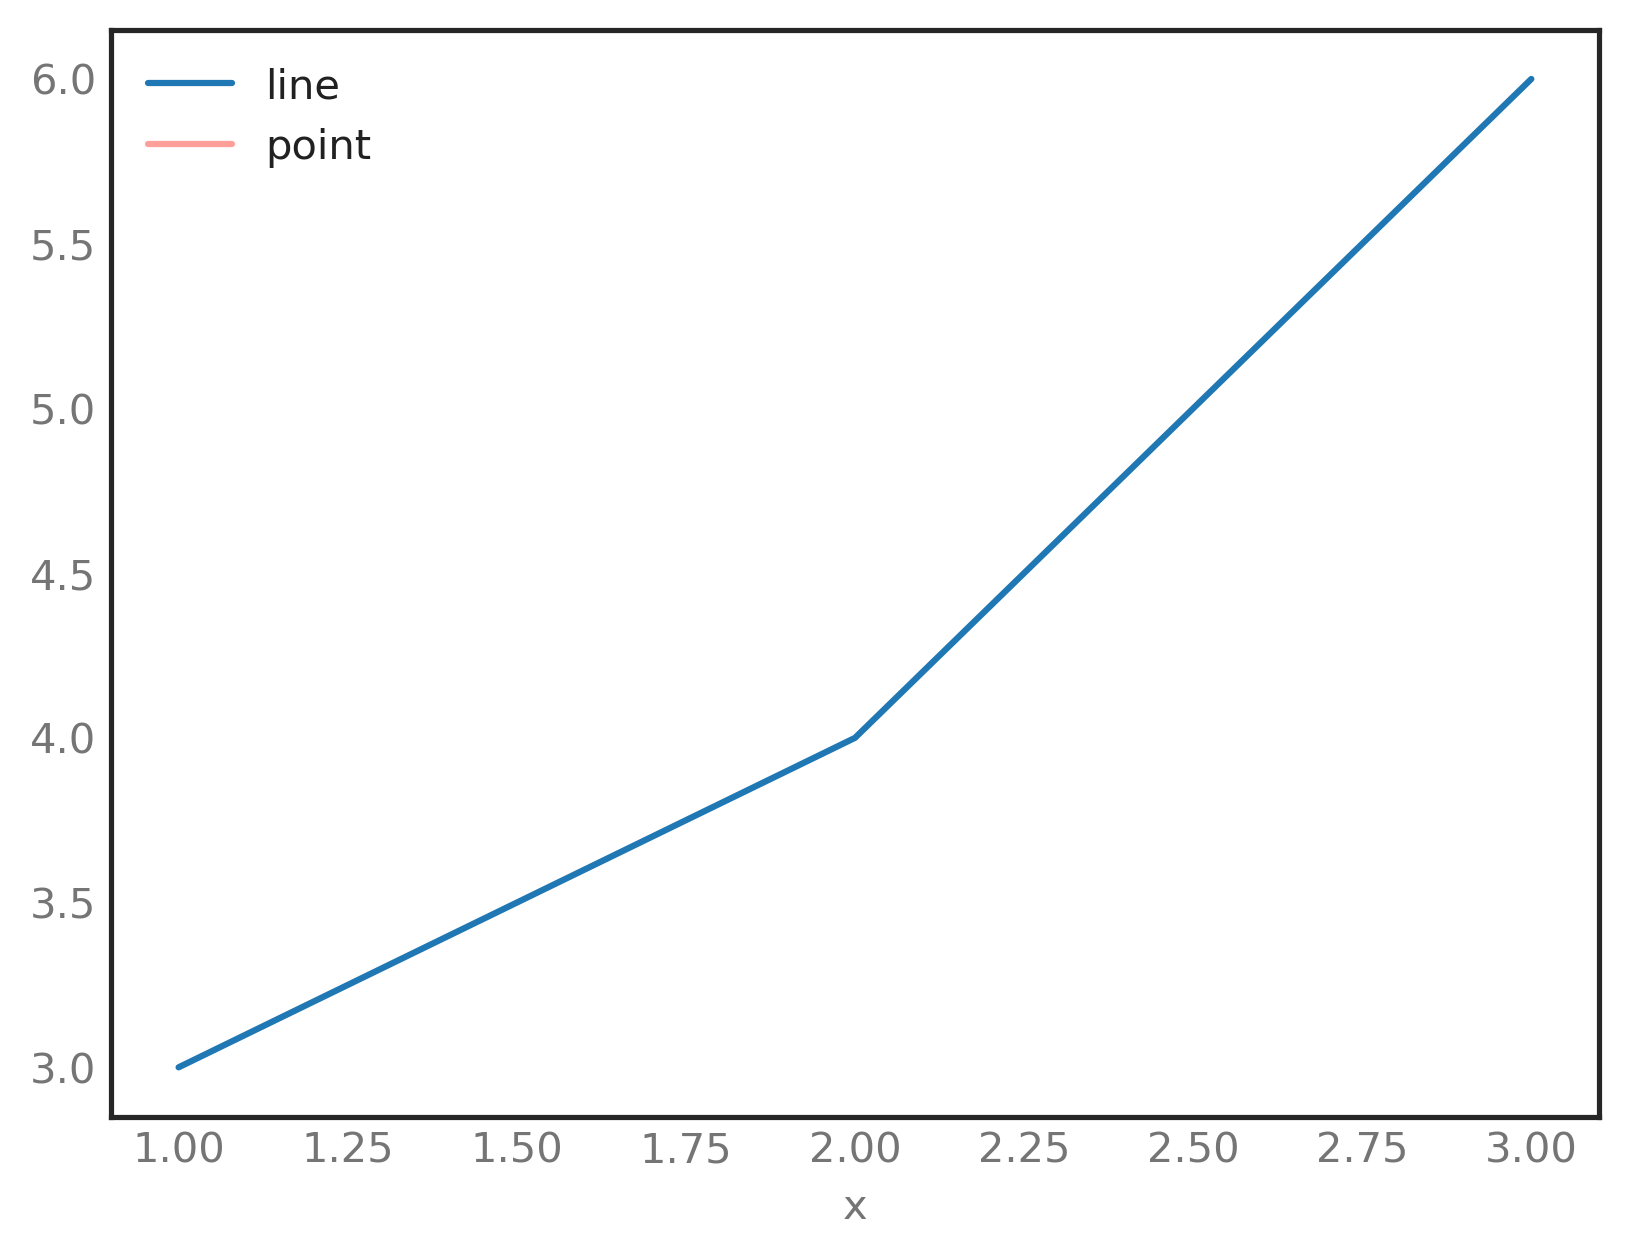
\includegraphics[width=13cm,keepaspectratio,]{images/plot-example.png}}
\caption{Example of a random plot}
\label{fig:plot}
\end{figure}

An example of a Table \ref{tab:regr}
\begin{table}[h]
\begin{center}

\begin{tabular}{L{2.5cm}L{2cm}L{2cm}L{2cm}L{2cm}}
\toprule 
Descriptives       & Mean & Standard Deviation & Minimum & Maximum \\ \hline
Team size               & 3.28      & 1.05   & 2              & 8             \\
Technical complexity & 4.82      & 3.02                & 1             & 18             \\
Winning      & 0.21     & 0.32                & 0             & 0.9            \\
Skill diversity         &  0.51     &  0.18               & 0              & 0.8            \\
Skill matching         & 0.25      & 0.22             & 0             & 1             \\
Team familiarity         & 0.08      & 0.3           & 0            & 3            \\
Preparation             & 0.25      & 0.43                & 0             & 1            \\
Hackathon experience      & 1.73     & 1.31           & 0.5             & 17            \\
Continuation intentions      & 0.60     & 0.49           & 0             & 1            \\ \bottomrule
\end{tabular}
\end{center}

\caption{Example Table.}
\label{tab:regr}
\end{table}
    \chapter{Related Work}
\label{sec:Related_Work}

Provide in brief the background information for your work/field keeping in mind that maybe your readers do not have experience with topics your reference or address in your thesis. 

In the second part, provide a review of the state of the art relevant to your thesis. Here you present relevant research that relates to your work. 

    \chapter{Methodology}
\label{sec:Methodology}

Here you should present how you aimed to answering your question or solving the problem you identified in the introduction.
You should present the methods and the instrument you use, the structure of your study or workplan and how you achieved the desirable outcome.

\section{Data collection}

\section{Study setup}

\section{Data analysis}


    \chapter{Results}
\label{sec:Results}

Here you present the results of your study (if you carried out one), and any data analysis you may have performed to answer your question.

    \chapter{Conclusion}
\label{sec:Conclusion}

In the Conclusions section you should elaborate on the following points:
\section{Discussion}
1. Conclusions: summarize your main objective/question/problem and how you solved it
\section{Theoretical and Practical Implications}
2. Summary of Contributions: explain what is your contribution and how it promotes knowledge in the field
\section{Limitations}
3. Limitations: Present the limitations or shortcomings of your work
\section{Future Work}
4. Future Research: Propose related topics that should be addressed by research in the future or ideas that you had while conducting your thesis. 


    
%Figures, tables and references
    \cleardoublepage
    \listoffigures
    \listoftables

%\bibliographystyle{acm}
 %   \bibliography{references}
  \printbibliography      
%appendices    

    \cleardoublepage
    \pagenumbering{roman}
    \appendix
    % !TeX root = main.tex

\chapter{Insert Appendix Name}
\section{Insert subtitle}


\end{document}
